%%% PostgreSQL is Web Scale, Open World Forum, 4/10/2013, 10h
%%%
%%% We call it the world's most advanced open source database, and we are
%%% actually offering in the same package full ACID compliance per default
%%% and advanced trade-offs to reach any kind of flexibility needed, all
%%% with per-transaction controls. That's including your replication and
%%% High Availability setup. Given proper use of those controls and some
%%% schemaless extensions, PostgreSQL really is web scale!

\documentclass{beamer}

\usepackage[utf8]{inputenc}

\usepackage{beamerthemesplit}
\usetheme{Boadilla}
\setbeamertemplate{itemize items}{\checkmark}
\beamertemplatetransparentcovered

\usepackage{multicol}

\title{PostgreSQL is web scale}
\subtitle{Open World Forum 2013}
\author{Dimitri Fontaine \texttt{dimitri@2ndQuadrant.fr}}
\date{October, 4 2013}
\logo{
\includegraphics[height=0.4cm]{2ndQuadrant-cross.png}}

\begin{document}

\frame{\titlepage}

\begin{frame}[fragile]
  \frametitle{Dimitri Fontaine}

  \begin{center}
    \textbf{2ndQuadrant France}
    \linebreak
    PostgreSQL Major Contributor
  \end{center}
  \vfill

\begin{columns}[c]
\column{.75\textwidth} 

  \begin{itemize}
   \item \texttt{pgloader}, \texttt{prefix}, \texttt{skytools}, …
   \item \texttt{apt.postgresql.org}
   \item \texttt{\textbf{CREATE EXTENSION}}
   \item \texttt{\textbf{CREATE EVENT TRIGGER}}
   \item MySQL migration tool, new \texttt{pgloader} version
  \end{itemize}  

\column{.25\textwidth}
\begin{center}
  
\includegraphics[height=7em]{2ndQuadrant-cross.png}
\end{center}
\end{columns}
\end{frame}

\section{PostgreSQL History}

\begin{frame}[fragile]
  \frametitle{What is PostgreSQL?}

  \center{PostgreSQL has roots in Database History}

\begin{columns}[c]
\column{.55\textwidth} 

  \begin{itemize}
  \item \textbf{UC Berkeley}
  \item 1973 INGRES
  \item 1986 Postgres
  \item 1996 PostgreSQL, Open Source BSD Licence
  \end{itemize}

\column{.45\textwidth}
\begin{center}
  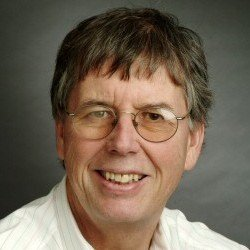
\includegraphics[height=7em]{021909_Stonebraker_Michael_250_large.jpg}
  \linebreak
  Michael Stonebraker
\end{center}
\end{columns}
\end{frame}

\begin{frame}[fragile]
  \frametitle{Project organisation}

  \center{Core team, Committers, Contributors, Sponsors}

\begin{columns}[c]
\column{.55\textwidth} 

  \begin{itemize}
  \item Contributors, Enterprises, Sponsors
  \item Mailing lists
  \item Release Model
  \item Minor and Major Versions
  \item Stable Versions, Current Versions
  \end{itemize}

\column{.45\textwidth}
\begin{center}
  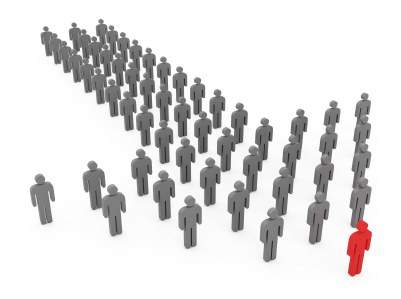
\includegraphics[height=7em]{elite_contributors.jpg}
\end{center}
\end{columns}
\end{frame}

\begin{frame}[fragile]
  \frametitle{Pace of development}

  \center{Thanks to a very active \textbf{community}, PostgreSQL is moving \textit{real fast.}}
  \vfill

\begin{columns}[c]
\column{.65\textwidth} 

  \begin{itemize}
  \item Catch-up with alternatives mainly has been done already
  \item Too many patches: Commit Fests
  \item Very fast innovation
  \item Yearly release cycle
  \end{itemize}

\column{.35\textwidth}
\begin{center}
  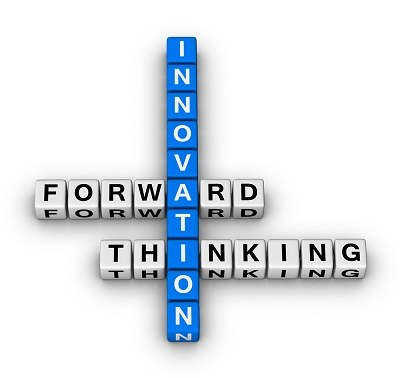
\includegraphics[height=10em]{innovation.jpg}
\end{center}
\end{columns}
\end{frame}

\begin{frame}[fragile]
  \frametitle{Strong Selling Points}

  \center{PostgreSQL strenghts make it disruptive}
  \vfill

\begin{columns}[c]
\column{.5\textwidth} 

  \begin{itemize}
  \item Fully ACID
  \item \textbf{trusted data}
  \item \textbf{transactions}
  \item \textbf{durability}
  \item \textbf{Crash Safety}
  \end{itemize}

\column{.5\textwidth}

  \begin{itemize}
  \item Query planner and optimizer
  \item Advanced Indexing
  \item Procedure Languages
  \item Extensibility (data types, functions, operators, indexes)
  \end{itemize}
\end{columns}

\vfill

\begin{center}
  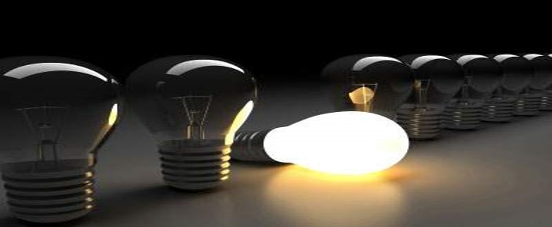
\includegraphics[height=8em]{disruptive-innovationn.jpg}
\end{center}
\end{frame}

\section{NoSQL}

\begin{frame}[fragile]
  \frametitle{Understanding NoSQL}

  \center{The NoSQL Offering, simplified}
  \vfill

\begin{columns}[c]
\column{.5\textwidth} 

  \begin{itemize}
  \item \textbf{API} rather than SQL
  \item No Schemas
  \item is ACID \textbf{fast enough}?
  \item Sharding and Multi Nodes Setup
  \end{itemize}

\column{.35\textwidth}
\begin{center}
  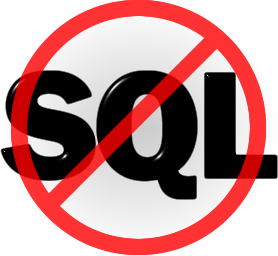
\includegraphics[height=8em]{nosql.png}
\end{center}
\end{columns}
\end{frame}

\section{Modern PostgreSQL}

\frame{
  \frametitle{Performances}

  \begin{center}
    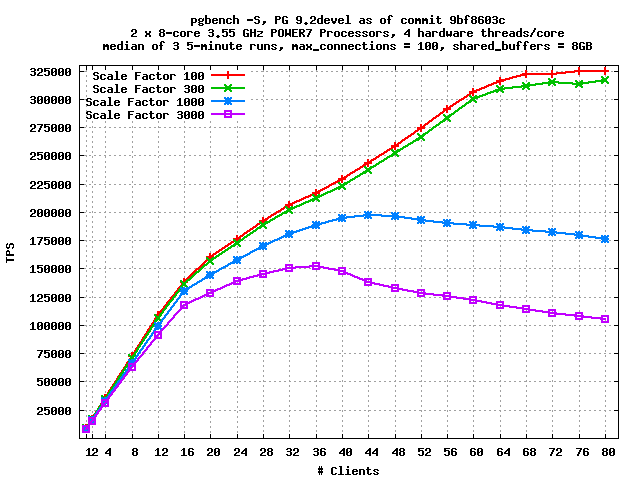
\includegraphics[height=20em]{read-scaling-power.png}
  \end{center}
}

\frame{
  \frametitle{Performances}

  \begin{center}
    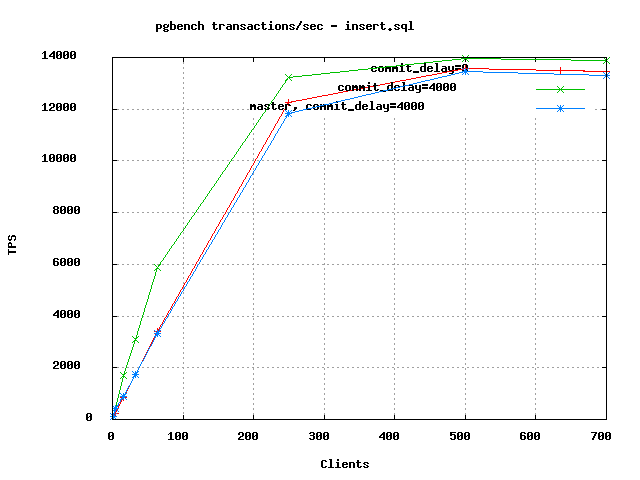
\includegraphics[height=20em]{insert_w_master_delay.png}
  \end{center}
}

\begin{frame}[fragile]
  \frametitle{Schemaless development with PostgreSQL}

  \center{PostgreSQL welcomes Engineers without a plan}
  \vfill

\begin{columns}[c]
\column{.35\textwidth} 

  \begin{itemize}
  \item hstore
  \item XML
  \item JSON
  \item PL/V8
  \item Indexing
  \end{itemize}  

\column{.65\textwidth}
\begin{center}
  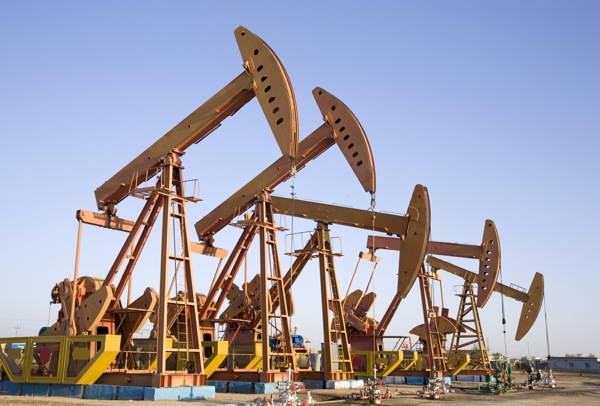
\includegraphics[height=12em]{Data-is-the-new-oil-Concentra.jpg}
  \linebreak
  Data is the New Oil!
\end{center}
\end{columns}
\end{frame}

\begin{frame}[fragile]
  \frametitle{Durability trade-offs}

  \center{When availability is about service, not data}
  \vfill

\begin{columns}[c]
\column{.55\textwidth} 

  \begin{itemize}
  \item Sometimes disks are just too slow
  \item \texttt{synchronous\_commit = off}
  \item Per Transaction Control
  \end{itemize}  

\column{.45\textwidth}
\begin{center}
  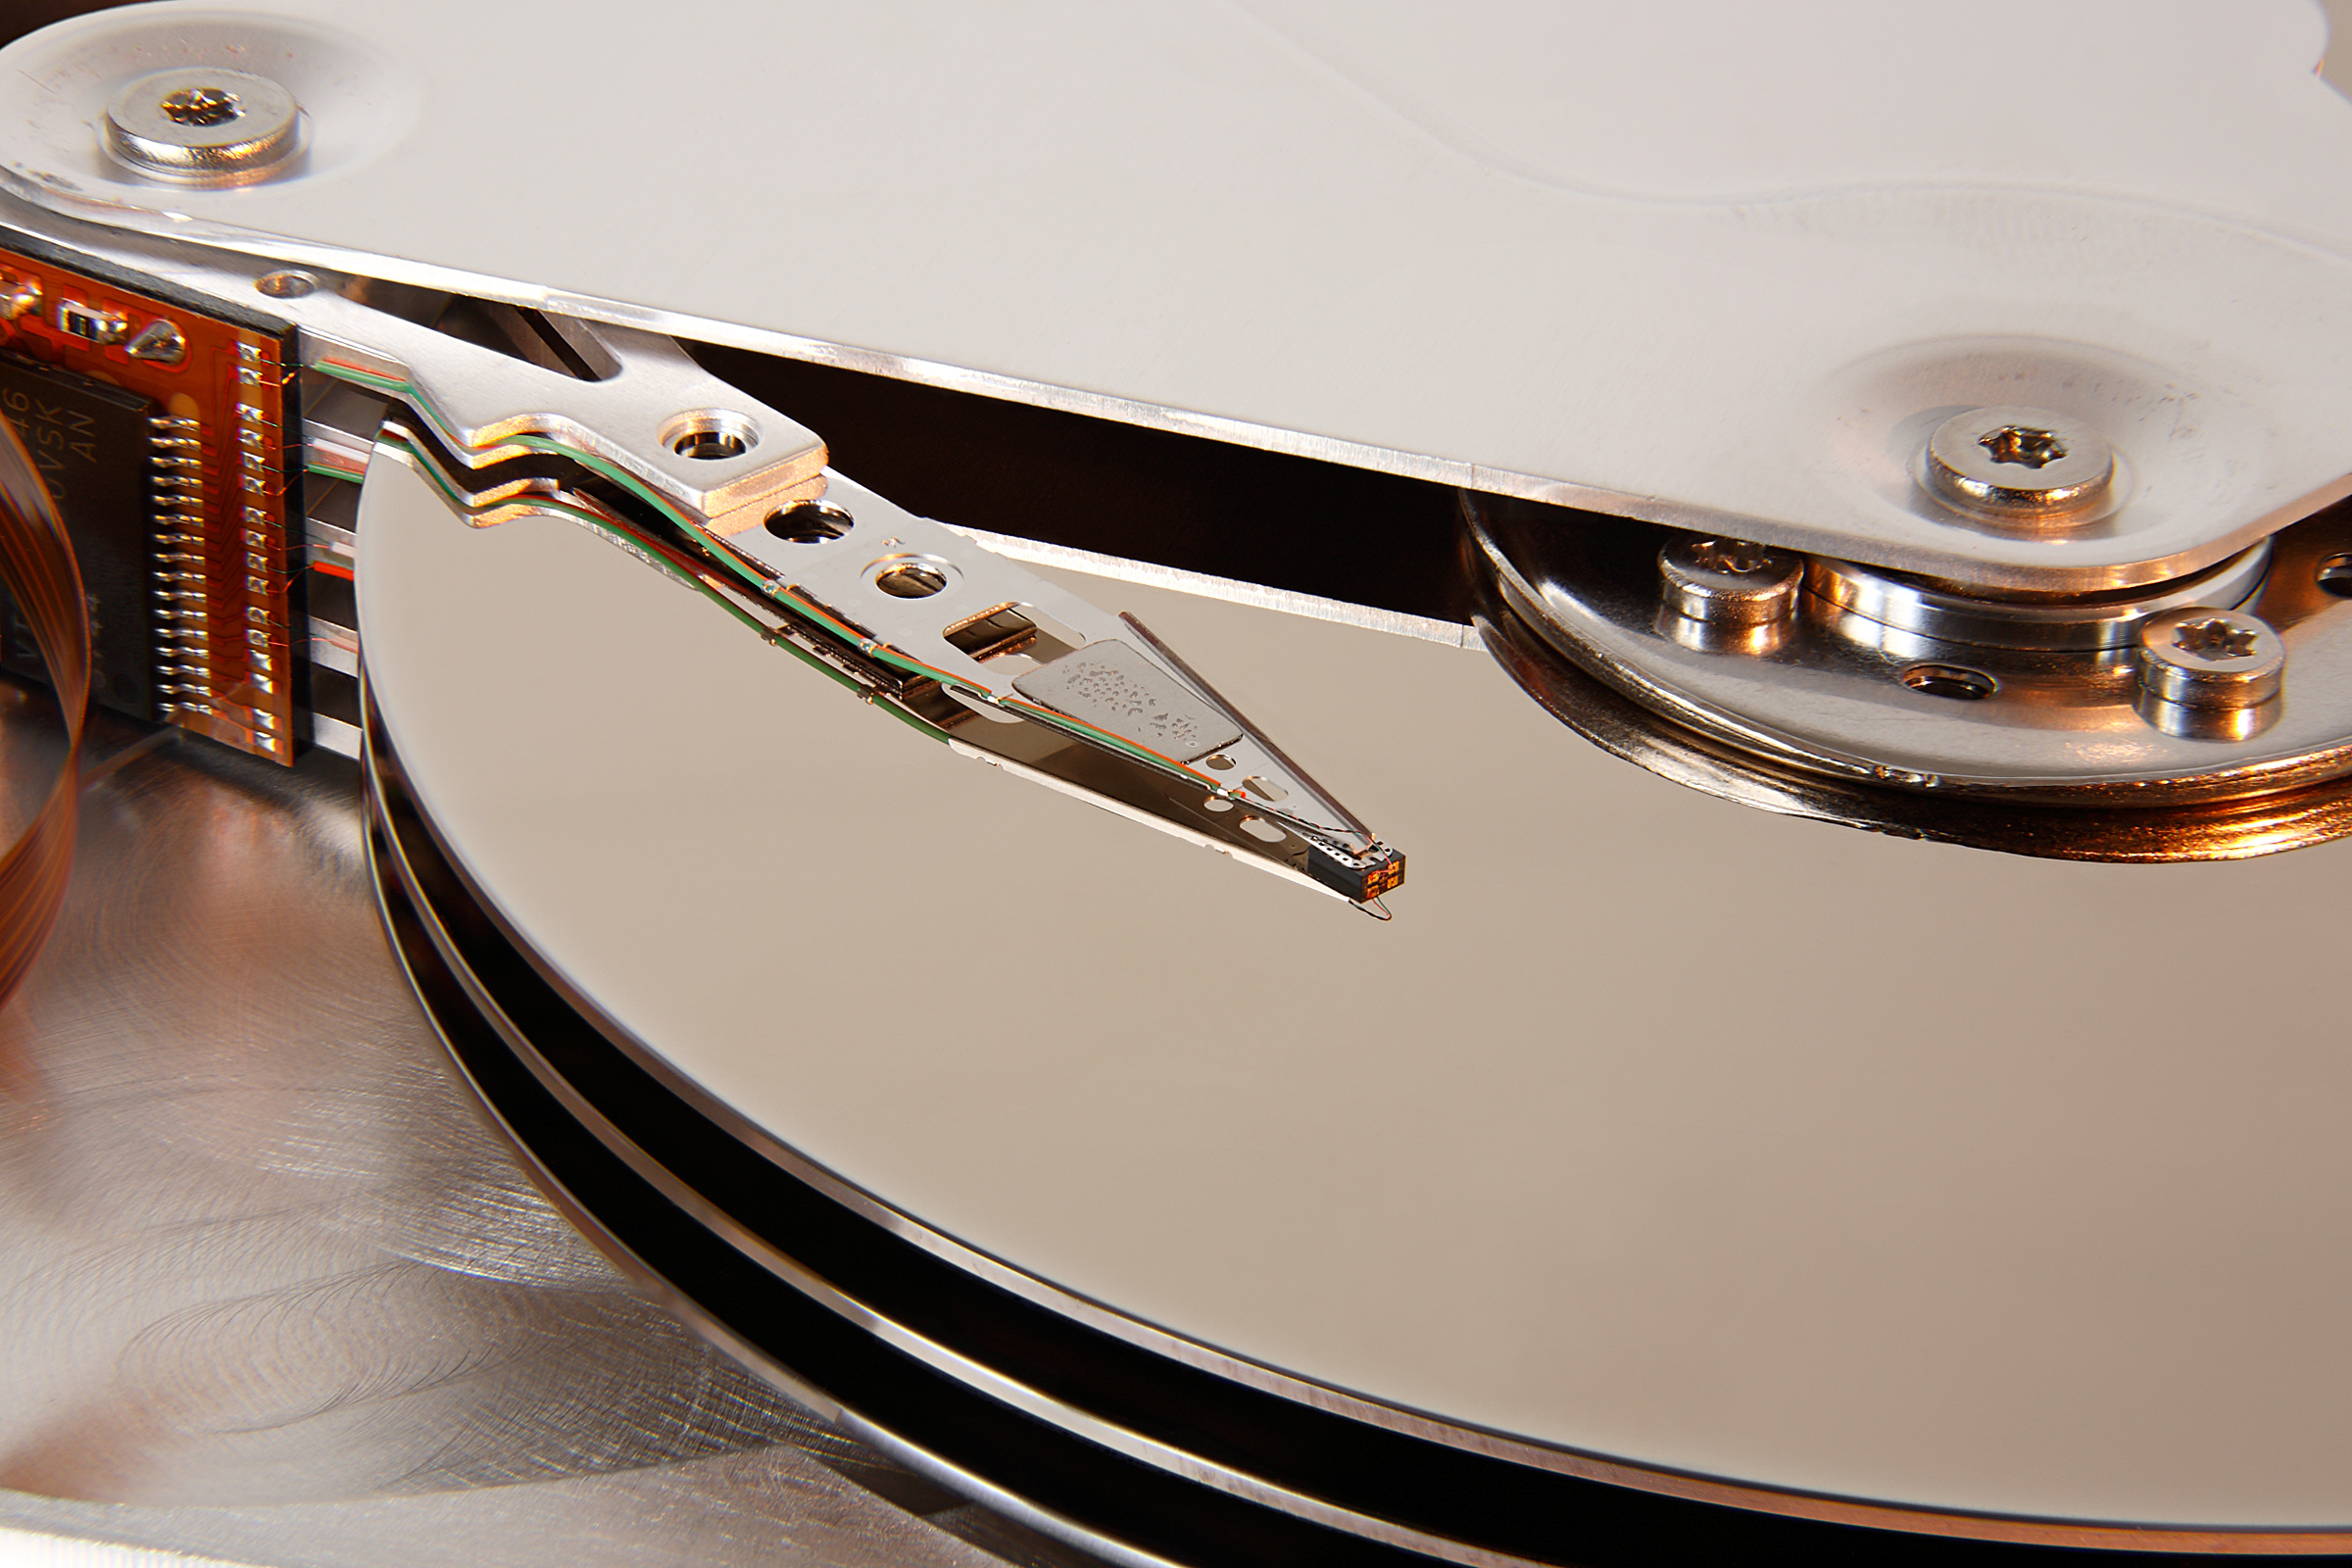
\includegraphics[height=8em]{Seagate_ST33232A_hard_disk_head_and_platters_detail.jpg}
\end{center}
\end{columns}

\vfill
  \begin{center}
    {Enable \textbf{Synchronous Replication} from within a trigger!
  \end{center}
\end{frame}

\begin{frame}[fragile]
  \frametitle{Asychronous Notifications}

  \center{Don't buzy loop until it changes, process incoming messages.}
  \vfill

\begin{columns}[c]
\column{.55\textwidth} 

  \begin{itemize}
  \item Pooling is not effective
  \item Receive messages when something happens
  \item \texttt{LISTEN}
  \item \texttt{NOTIFY}
  \item Send a JSON payload!
  \end{itemize}

\column{.45\textwidth}
\begin{center}
  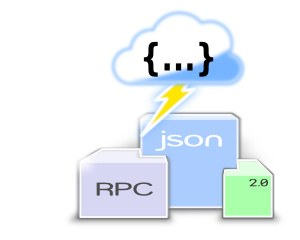
\includegraphics[height=8em]{masthead-jsonrpc2base.jpg}
\end{center}
\end{columns}
\end{frame}

\section{Conclusion}

\frame{
  \frametitle{PostgreSQL is YeSQL!}

\begin{center}
  Yes, it really is. Welcome to YeSQL!
  \vfill

  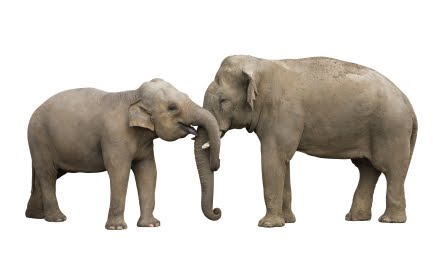
\includegraphics[height=9em]{elephant_upgrade.jpg}
\end{center}
}

\frame{
  \frametitle{Questions?}

\begin{center}
  Now is the time to ask!
  \vfill

  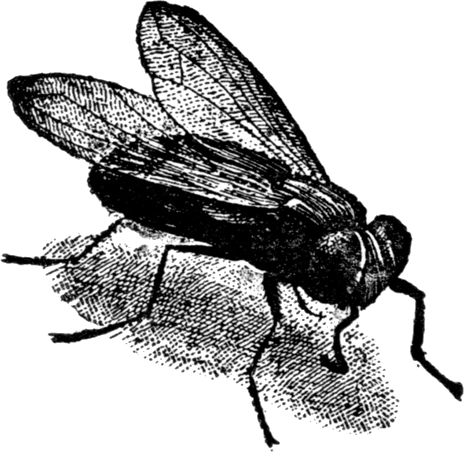
\includegraphics[height=9em]{fly.png}
\end{center}
}

\end{document}
